%%%%%%%%%%%%%%%%%%%%%%%%%%%%%%%%%%%%%%%%%
% Short Sectioned Assignment LaTeX Template Version 1.0 (5/5/12)
% This template has been downloaded from: http://www.LaTeXTemplates.com
% Original author:  Frits Wenneker (http://www.howtotex.com)
% License: CC BY-NC-SA 3.0 (http://creativecommons.org/licenses/by-nc-sa/3.0/)
%%%%%%%%%%%%%%%%%%%%%%%%%%%%%%%%%%%%%%%%%

%----------------------------------------------------------------------------------------
%	PACKAGES AND OTHER DOCUMENT CONFIGURATIONS
%----------------------------------------------------------------------------------------

\documentclass[paper=a4, fontsize=11pt]{scrartcl} % A4 paper and 11pt font size

% ---- Entrada y salida de texto -----

\usepackage[T1]{fontenc} % Use 8-bit encoding that has 256 glyphs
\usepackage[utf8]{inputenc}
%\usepackage{fourier} % Use the Adobe Utopia font for the document - comment this line to return to the LaTeX default


\usepackage[utf8]{inputenc}
\usepackage[T1]{fontenc}
\usepackage[spanish]{babel}
\usepackage{times}

\usepackage{color}
\definecolor{gray97}{gray}{.97}
\definecolor{gray75}{gray}{.75}
\definecolor{gray45}{gray}{.45}

\usepackage{listings}
\lstset{ frame=Ltb,
	framerule=0pt,
	aboveskip=0.5cm,
	framextopmargin=3pt,
	framexbottommargin=3pt,
	framexleftmargin=0.4cm,
	framesep=0pt,
	rulesep=.4pt,
	backgroundcolor=\color{gray97},
	rulesepcolor=\color{black},
	%
	stringstyle=\ttfamily,
	showstringspaces = false,
	basicstyle=\small\ttfamily,
	commentstyle=\color{gray45},
	keywordstyle=\bfseries,
	%
	numbers=left,
	numbersep=15pt,
	numberstyle=\tiny,
	numberfirstline = false,
	breaklines=true,
}

% minimizar fragmentado de listados
\lstnewenvironment{listing}[1][]
{\lstset{#1}\pagebreak[0]}{\pagebreak[0]}

\lstdefinestyle{consola}
{basicstyle=\scriptsize\bf\ttfamily,
	backgroundcolor=\color{gray75},
}

\lstdefinestyle{C}
{language=C,
}
% ---- Idioma --------

\usepackage[spanish, es-tabla]{babel} % Selecciona el español para palabras introducidas automáticamente, p.ej. "septiembre" en la fecha y especifica que se use la palabra Tabla en vez de Cuadro
% ---- Otros paquetes ----

\usepackage{amsmath,amsfonts,amsthm} % Math packages
%\usepackage{graphics,graphicx, floatrow} %para incluir imágenes y notas en las imágenes
\usepackage{graphics,graphicx, float} %para incluir imágenes y colocarlas

% Para hacer tablas comlejas
%\usepackage{multirow}
%\usepackage{threeparttable}

%\usepackage{sectsty} % Allows customizing section commands
%\allsectionsfont{\centering \normalfont\scshape} % Make all sections centered, the default font and small caps

\usepackage{fancyhdr} % Custom headers and footers
\pagestyle{fancyplain} % Makes all pages in the document conform to the custom headers and footers
\fancyhead{} % No page header - if you want one, create it in the same way as the footers below
\fancyfoot[L]{} % Empty left footer
\fancyfoot[C]{} % Empty center footer
\fancyfoot[R]{\thepage} % Page numbering for right footer
\renewcommand{\headrulewidth}{0pt} % Remove header underlines
\renewcommand{\footrulewidth}{0pt} % Remove footer underlines
\setlength{\headheight}{13.6pt} % Customize the height of the header

\numberwithin{equation}{section} % Number equations within sections (i.e. 1.1, 1.2, 2.1, 2.2 instead of 1, 2, 3, 4)
\numberwithin{figure}{section} % Number figures within sections (i.e. 1.1, 1.2, 2.1, 2.2 instead of 1, 2, 3, 4)
\numberwithin{table}{section} % Number tables within sections (i.e. 1.1, 1.2, 2.1, 2.2 instead of 1, 2, 3, 4)

\setlength\parindent{0pt} % Removes all indentation from paragraphs - comment this line for an assignment with lots of text

\newcommand{\horrule}[1]{\rule{\linewidth}{#1}} % Create horizontal rule command with 1 argument of height


\begin{document}
\title{
\normalfont \normalsize 
\textsc{{\bf Metaheurísticas (2015-16) \\ Grado en Ingeniería Informática \\ Universidad de Granada} \\ [25pt] % Your university, school and/or department name(s)
\horrule{0.5pt} \\[0.4cm] % Thin top horizontal rule
\huge Práctica 3: Búsquedas con técnicas basadas en poblaciones: Algoritmos genéticos. \\ % The assignment title
\horrule{2pt} \\[0.5cm] % Thick bottom horizontal rule
}}
\author{Miguel López Campos\\ 54120359W\\ miguelberja@correo.ugr.es\\ Grupo Viernes 18:30} % Nombre y apellidos


\date{\normalsize\today} % Incluye la fecha actual
%----------------------------------------------------------------------------------------
% DOCUMENTO
%----------------------------------------------------------------------------------------


	
	\maketitle % Muestra el Título
	\newpage %inserta un salto de página
	
	\tableofcontents % para generar el índice de contenidos
	\listoffigures

	
	\newpage
	
	\
	
	
	
	\section{Descripción del problema}
	El problema que estamos abordando es la selección de características. Este problema es muy útil en el campo de "machine learning".
	\\
	\\
	Tenemos un conjunto de datos de entrenamiento y otro de validación, ambos etiquetados o clasificados. Lo que queremos hacer es 'aprender' una función que a partir de las características del conjunto de datos de entrenamiento, nos permita estimar el etiquetado de otros vectores de características. Lo que nosotros queremos hacer es eliminar las características que no son relevantes en el problema, eliminando de esta manera ruido en el conjunto de datos y mejorando la eficiencia de nuestro clasificador. Es decir, no sólo mejoraremos el tiempo, si no muy probablemente la calidad de nuestras soluciones también (en cuanto al error se refiere).
	\\
	\\
	La gran dificultad de este problema radica en el gran número de soluciones posibles, llevándonos al punto de que un algoritmo Greedy que nos garantice la solución óptima podría llevarnos días de ejecución para determinados problemas. Es por esto por lo que tenemos que usar Metaheurísticas. Necesitamos soluciones buenas (aunque no sea la mejor) en un tiempo menor.
	\\
	\\
	Nosotros usaremos para clasificar el algoritmo 3NN. Lo que hace este algoritmo es calcular la distancia euclídea entre el vector de características al cual queremos estimar una clase y el resto de vectores de características del conjunto de entrenamiento. Lo que hace el 3NN es coger los 3 elementos menos distantes y la clase mayoritaria entre esos 3 será la estimación que haremos.
	\\
	\\
	Validaremos con la técnica 5x2 Cross Validation. Usaremos 5 particiones de los datos distintas al 50\% (y aleatorias) y aprenderemos el clasificador con una submuestra y validaremos con la otra y después al contrario. Con esta técnica tendremos el porcentaje de acierto, que nos servirá para ver la calidad de nuestro algoritmo.
	\\
	\\
	Otros datos con los que valoraremos la calidad de nuestros algoritmos serán los tiempos de ejeución y los porcentajes de reducción, es decir, el porcentaje de características que hemos reducido.
	\\
	\\
	Con nuestras metaheurísticas querremos optimizar la función de acierto. Es decir, queremos maximizar el acierto, siendo la función:\\
	$tasaclass = 100*\frac{nºinstancias bien clasificadas}{nº instancias Total}$
	
	\newpage
	
	
	\section{Descripción de los aspectos comunes de los algoritmos}
	La práctica ha sido desarrollada en C++.
	\\
	
	\begin{enumerate}
		\item Representación de las soluciones. Para representar las soluciones utilizaremos un array de booleanos. Será común a todos los algoritmos. Si la componente $i$ es true, esto indicará que la característica $i$ se tendrá en cuenta (no ha sido eliminada).
		
		\item Función objetivo. La función que queremos optimizar se trata del porcentaje de acierto de estimaciones de clases, descrita en el apartado anterior.
		\\
		\\
		En pseudocódigo es la siguiente:
		\begin{lstlisting}
funcion_objetivo(conjunto_training, caracteristicas_activas)
begin
  Para todo elemento i del conjunto_test
  begin
    elemento <- elemento i del conjunto_training
	clase <- 3NN(conjunto_training-{elemento}, elemento, caracteristicas_activas)
				
	Si la clase estimada por 3NN se corresponde a la clase real -> aciertos++
  end
			
  promedio <- aciertos/tamaño conjunto_test
			
  devolver promedio
end
		\end{lstlisting}
		
		\item Función clasificadora. Como función clasificadora usaremos el algoritmo 3NN, descrito anteriormente.
		\\
		\\
		\newpage
		
		El pseudocódigo es el siguiente:
		\begin{lstlisting}
3NN(conjunto_training, vector_caracteristicas, caracteristicas_activas)
begin
  Para cada vector i de caracteristicas de training
  begin
  
    array_distancias.añadir(distanciaeuclidea(i, vector_caracteristicas, caracteristicas_activas))
    
   end
   
  minimo1 <- minimo(array_distancias)
  minimo2 <- minimo(array_distancias-minimo1)
  minimo3 <- minimo(array_distancias-minimo1-minimo2)
  
  Si la clase de vector_caracteristicas[minimo2]==clase de vector_caracteristicas[minimo3] entonces
    La clase del vector de caracteristicas es esa
  Si no
    La clase del vector de caracteristicas es la clase de vector_caracteristicas[minimo1]
    
  devolver clase del vector de caracteristicas
  
end
		\end{lstlisting}
		
		\item Función para la generación de soluciones aleatorias
\begin{lstlisting}
PRE: solucion está inicialmente entero a falso

Generar_solucion_aleatoria(solucion, tamanio_solucion)
begin
  indices_disponibles <- [0...tamanio_solucion-1]
  caracteristicas_a_cambiar <- Random(0, tamanio_solucion-1)
  
  Para i=0 hasta caracteristicas_a_cambiar
  begin
    caracteristica <- Random(0, indices_disponibles.length-1)
    solucion[indices_disponibles[caracteristica]] <- true
    indices_disponibles-{caracteristica}    //Elimino el indice de la caracteristica para no volver a cambiarla
  end
  
  devolver solucion
end

\end{lstlisting}
		
		\item Antes de trabajar con cualquier algoritmo hay que normalizar los conjuntos de datos.
		
		\item El criterio de parada para los algoritmos genéticos es que realicen 15000 evaluaciones de la función objetivo.
		
		\item Para reducir los tiempos he seguido las recomendaciones del seminario. En el modelo generacional, para decidir si una pareja cruza o no, he calculado el número esperado de cruces (la esperanza matemática) y he realizado ese número (Probabilidad de cruce * (Número de cromosomas/2)). Igual para la mutación, donde he calculado el número de mutaciones esperado y he realizado las mutaciones a cromosomas aleatorios y genes aleatorios. Para emparejar he aprovechado la aletoriedad en la fase de selección.
		
		
		\item Para cada algoritmo he plantado el mismo valor de semilla para una correspondiente iteración.
		
		\item He usado para tomar tiempos y para crear números aleatorios las funciones dadas en decsai.
	\end{enumerate}
	
	\section{Algoritmo de comparación SFS}
	El algoritmo de comparación SFS es muy simple. Primero se genera una solución con todo a
	falso. A partir de aquí, exploramos todo el vector solución y cogemos la característica con la que
	vayamos a obtener mayor ganancia. Una vez la escojamos, volvemos a realizar otra iteración cogiendo la siguiente característica que nos de más ganancia y así sucesivamente. El algoritmo acaba cuando ya no haya mejora en una búsqueda completa sobre el vector solución.
	\\
	\\
	La descripción en pseudocódigo del algoritmo es la siguiente:
	\begin{lstlisting}
SFS(training, Solucion, Tasa_Solucion)
begin
  mejor_solucion <- 0.0
  mejora <- true
  
  Mientras mejora
  begin
    mejora <- false
    S_tmp <- Solucion
    
    Para i=0 hasta S_tmp.length
    begin
      Si S_tmp[i] es false entonces
        S_tmp[i] <- true
        S_tmp_tasa <- funcion_objetivo(training, S_tmp)
        
        Si S_tmp_tasa es mejor que mejor_solucion entonces
          mejor_solucion <- S_tmp_tasa
          mejora <- true
          Solucion <- S_tmp
          
        S_tmp[i] <- false
    end
  end
  
  devolver Solucion y mejor_solucion //Por referencia
  
end
	\end{lstlisting}


	\section{Algoritmo genético generacional}
	En los algoritmos genéticos generacionales, en cada nueva iteración, se reemplaza toda la población por la nueva.
	Los parámetros usados son 0.7 para la probabilidad de cruce y 0.001 para la probabilidad de mutación. Ambas probabilidades son las dadas por el guión de la práctica. Como criterio de parada he puesto que se realicen un máximo de 15000 evaluaciones de la función objetivo. Para mantener el elitismo, me aseguro de que la mejor solución de una población anterior se encuentra en la nueva población cambiándola por la peor de esta última (en el caso de que sea mejor).
	\\
	\\
	El mecanismo de selección que he empleado consiste en realizar tantos concursos binarios aleatorios como cromosomas hay en la población (en nuestro caso 30). Los ganadores de estos concursos binarios serán los cromosomas de nuestra población seleccionada. La descripción en pseudocódigo es la siguiente:
	
	\begin{lstlisting}
seleccionar(poblacion, tasas_poblacion, seleccion, tasas) //Por referencia 
begin
  seleccion <- Array() //Array de cromosomas (vectores solucion)
  tasas <- Array() //Tasas de los seleccionados
  
  disponibles <- 0..poblacion.length-1 //Array de índices para controlar que no compite un cromosoma consigo mismo
  
  Para i=0 hasta poblacion.length
  begin
    aux <- disponibles
    
    random1 <- Random(0, aux.length-1) //Random devuelve un entero
    aux <- aux-{random1} //Me aseguro de que no cojo el mismo cromosoma
    random2 <- Random(0, aux.length-1)
    
    aux <- disponibles
    
    Si tasas_poblacion[random1] es mejor que tasas_poblacion[random2] entonces
      seleccion.aniadir(poblacion[random1])
      tasas.aniadir(tasas_poblacion[random1])
    si no entonces
      seleccion.aniadir(poblacion[random2])
      tasas.aniadir(tasas_poblacion[random2])
    
  end
  
  devolver seleccion y tasas //Por referencia
  
end
	\end{lstlisting}
	
Para la fase de cruce lo que hago es de la selección obtenida de la fase de selección, cruzo el primero con el segundo, el segundo con el tercero, etc. hasta cubrir el número esperado de cruces, calculado con la fórmula $ProbabilidadCruce * (NumeroCromosomas/2)$. Lo que hago es elegir dos puntos de corte (asegurándome de que no son el mismo porque si no no cruzarían nada) y los elementos del cromosoma (o vector solución) que están entre esos dos puntos de corte son los que se intercambiarán un padre y otro, es decir, los nuevos cromosomas serán ellos mismos pero cada uno con la parte de central del otro. Estos puntos de corte además tienen que ir desde la segunda componente del array hasta la penúltima. La función de cruce es la siguiente:
\begin{lstlisting}
cruce(padre1, padre2) //por referencia
begin
  posibles <- 0..padre1.length-1 //Numero de caracteristicas del vector solucion
  
  corte1 <- posibles[Random(1, posibles.length-2)]
  posibles <- posibles-{corte1}
  corte2 <- posibles[Random(1, posibles.length-2)]
  
  Si corte1 > corte2 entonces
    hago swap entre corte1 y corte2
    
  aux1 <- padre1[corte1..corte2] //Cojo la parte central del array
  aux2 <- padre2[corte1..corte2]
  
  padre1 <- padre1-padre1[corte1..corte2] //Elimino la parte central del array
  padre2 <- padre2-padre2[corte1..corte2]
  
  padre1.insertar(aux2, corte1) //Inserto la parte central del otro padre a partir de cote1
  padre2.insertar(aux1, corte1)
  
  
  devolver padre1 y padre2 //por referencia
  
end
\end{lstlisting}


Para la mutación, al igual que con los cruces, calculo el número esperado de mutaciones que se van a realizar. Para ello uso la fórmula $ProbabilidadMutacion * numeroCromosomas * numeroGenes$. Siendo la probabilidad de mutación 0.001. La función con la que muto es la siguiente:

\begin{lstlisting}
mutar(solucion, i) //Muto la componente i de solucion
begin
  Si solucion[i] es true entonces lo pongo a false
  si no lo pongo a true
  
  devolver solucion
  
end
\end{lstlisting}

El algoritmo completo en pseudocódigo es el siguiente:
\begin{lstlisting}
//PRE: Solucion inicialmente es entero falso

AGG(training, Solucion, Tasa_Solucion)
begin
  poblacion <- Array() //Array de vectores solucion
  tasas_poblacion <- Array() //Array de las tasas de la poblacion
  
  Para i=0 hasta 30
  begin
    tmp <- generar_solucion_aleatoria(Solucion, Solucion.length)
    poblacion.aniadir(tmp)
    tasa <- funcion_objetivo(training, tmp)
    tasas_poblacion.aniadir(tasa)
  end
  
  
  Para i=0 hasta 15000
  begin
    //Guardo el mejor elemento de la poblacion
    indice_mejor <- maximo(tasas_poblacion)
    mejor <- poblacion[indice_mejor]
    
    Seleccion <- Array() //Array de vectores solucion
    Tasas_Seleccion <- Array() //Array de tasas
    
    
    //Fase de seleccion
    seleccionar(poblacion, tasas_polacion, Seleccion, Tasas_Seleccion) //Por referencia
    
    //Fase de cruce
    n_cruces <- 0.7*30/2
    
    Para j=0 hasta n_cruces
    begin
      padre1 <- Seleccion[2*j]
      padre2 <- Seleccion[2*j+1]
      
      cruce(padre1, padre2)
    end
    
    //Fase de mutación
    n_mutaciones <- 0.001*30*Seleccion[1].length
    
    Para j=0 hasta n_mutaciones
    begin
      r1 <- Random(0, Seleccion.length-1)
      r2 <- Random(0, Seleccion[r1].length-1)
      
      mutar(Seleccion[r1], r2)
    end
    
    
    //Fase de reemplazamiento
    Para j=0 hasta 30
    begin
      tasas_Seleccion[j] <- funcion_objetivo(training, seleccion[j])
    end
    
    encontrado <- Buscar(mejor) //Busco si está la mejor solucion anteriormente guardada
    
    Si !encontrado entonces
      min <- minimo(tasas_seleccion)
      
      Si tasas_seleccion[min] < tasas_poblacion[ind_mejor] entonces
        seleccion[min] <- mejor
        tasas_seleccion[min] <- tasas_poblacion[ind_mejor]
        
  end
  
  ind_max <- maximo(tasas_poblacion)
  solucion <- poblacion[ind_max]
  Tasa_Solucion <- Tasas_poblacion[ind_max]
  
  devolver solucion y Tasa_Solucion //Por referencia
  
end
\end{lstlisting}
NOTA: El incremento de la i en el bucle más externo lo hago de 30 en 30 ya que en cada iteración se realizan 30 evaluaciones de la función objetivo.

\section{Algoritmo genético estacionario}
En este modelo de algoritmo genético se eligen dos padres aleatorios de la población y se aplican los operadores genéticos sobre éstos. Este modelo es elitista y además tiene una convergencia rápida al reemplazar los peores cromosomas (soluciones) por otras mejores. En este modelo también usaremos como probabilidad de mutación 0.01 y la probabilidad de cruce será 1 ya que siempre se cruzarán los dos padres.
\\
\\
En la fase de selección realizo dos concursos binarios. En estos concursos controlaré que los que han participado en el primer concurso no participen en el segundo y además que un cromosoma no compita contra sí mismo. La selección la realizo con el siguiente pseudocódigo:
\begin{lstlisting}
seleccionar(poblacion, tasas_poblacion, padre1, padre2) //Por referencia 
begin
  posibles <- 0..poblacion.length-1 //No puedo repetir en los concursos el mismo elemento
  
  r1 <- Random(0,posibles.length-1)
  posibles <- posiles-{r1}
  r2 <- Random(0,posibles.length-1)
  posibles <- posiles-{r2}
  r3 <- Random(0,posibles.length-1)
  posibles <- posiles-{r3}
  r4 <- Random(0,posibles.length-1)

  posibles <- 0..poblacion.length-1
  
  Si tasas_poblacion[posibles[r1]] >= tasas_poblacion[posibles[r2]] entonces
    padre1 <- poblacion[posibles[r1]]
  si no entonces
    padre1 <- poblacion[posibles[r2]]
    
  Si tasas_poblacion[posibles[r3]] >= tasas_poblacion[posibles[r4]] entonces
  padre2 <- poblacion[posibles[r3]]
  si no entonces
  padre2 <- poblacion[posibles[r4]]
  
  devolver padre1 y padre2 //Por referencia
end
\end{lstlisting}
La fase de cruce la hago igual que en el modelo generacional. El pseudocódigo es el siguiente:

\begin{lstlisting}
cruce(padre1, padre2) //por referencia
begin
	posibles <- 0..padre1.length-1 //Numero de caracteristicas del vector solucion
	
	corte1 <- posibles[Random(1, posibles.length-2)]
	posibles <- posibles-{corte1}
	corte2 <- posibles[Random(1, posibles.length-2)]
	
	Si corte1 > corte2 entonces
	hago swap entre corte1 y corte2
	
	aux1 <- padre1[corte1..corte2] //Cojo la parte central del array
	aux2 <- padre2[corte1..corte2]
	
	padre1 <- padre1-padre1[corte1..corte2] //Elimino la parte central del array
	padre2 <- padre2-padre2[corte1..corte2]
	
	padre1.insertar(aux2, corte1) //Inserto la parte central del otro padre a partir de cote1
	padre2.insertar(aux1, corte1)
	
	
	devolver padre1 y padre2 //por referencia

end
\end{lstlisting}

La mutación también uso el mismo modelo que en el generacional:
\begin{lstlisting}
mutar(solucion, i) //Muto la componente i de solucion
begin
	Si solucion[i] es true entonces lo pongo a false
	si no lo pongo a true
	
	devolver solucion
end
\end{lstlisting}
La descripción en pseudcódigo del algoritmo completo (AGE) es la siguiente:
\begin{lstlisting}
//PRE: Solucion inicialmente es entero falso

AGG(training, Solucion, Tasa_Solucion)
begin
  poblacion <- Array() //Array de vectores solucion
  tasas_poblacion <- Array() //Array de las tasas de la poblacion

  Para i=0 hasta 30
  begin
    tmp <- generar_solucion_aleatoria(Solucion, Solucion.length)
    poblacion.aniadir(tmp)
    tasa <- funcion_objetivo(training, tmp)
    tasas_poblacion.aniadir(tasa)
  end


  Para i=0 hasta 15000
  begin
    padre1 <- Array solucion
    padre2 <- Array solucion
    
    //FASE DE SELECCIÓN
    seleccionar(poblacion, tasas_poblacion, padre1, padre2)
    
    //FASE DE CRUCE
    cruce(padre1, padre2)
    
    //FASE DE MUTACIÓN
    random1 <- Rand() //Numero aleatorio entre 0 y 1 sin incluir el 1
    random2 <- Rand()
    
    Si random1 <= 0.001 entonces
      r1 <- Random(0, padre1.length-1)
      mutar(padre1, r1)
    
    Si random2 <= 0.001 entonces
      r1 <- Random(0, padre2.length-1)
      mutar(padre2, r2)
      
    //FASE DE REEMPLAZAMIENTO
    tasa_padre1 <- funcion_objetivo(training, padre1)
    tasa_padre2 <- funcion_objetivo(training, padre2)
    
    min1 <- minimo(tasas_poblacion)
    min2 <- minimo(tasas_poblacion-tasas_poblacion[min2])
    
    Si tasa_padre2 >= tasa_padre1 entonces
      Hago swap entre padre1 y padre2
      
    Si tasa_padre1 >= tasas_poblacion[min1] entonces
      tasas_poblacion[min1] <- tasa_padre1
      poblacion[min1] <- padre1
      
      Si tasa_padre2 >= tasas_poblacion[min2] entonces
        tasas_poblacion[min2] <- tasa_padre2
        poblacion[min2] <- padre2
      
    si no si tasa_padre1 >= tasas_poblacion[min2] entonces
      tasas_poblacion[min2] <- tasa_padre1
      poblacion[min2] <- padre1
      
  end
  
  ind_max <- maximo(tasas_poblacion)
  Solucion <- poblacion[ind_max]
  Tasa_Solucion <- tasas_poblacion[ind_max]
  
  devolver Solucion y Tasa_Solucion //por referencia
  
end
    
\end{lstlisting}
NOTA: En el bucle más externo voy incrementando la i de 2 en 2 ya que en cada iteración se realizan 2 evaluaciones de la función objetivo.

\section{Aspectos técnicos de la práctica}
La práctica ha sido desarrollada en C++. El código ha sido implementado basándome en los
pseudocódigos de las transparencias de clase (adaptándolos al problema). Cada uno de los algoritmos está implementado en un cpp diferente. Dentro de estos cpp tenemos las funciones de
evaluación, así como de lectura de los ficheros de datos. Cada algoritmo por lo tanto se evaluará
en un ejecutable distinto. Para compilar el código simplemente hay que usar make (hay un makefile implementado) y en la carpeta bin se crearán los ejecutables. Cada ejecutable tendrá como
salida los datos de las ejecuciones de los algoritmos.
\\
\\
Los ficheros de datos que he usado son los que hay subidos en la plataforma de la asignatu-
ra, a excepción de movement\_libras, cuyo fichero de datos he tenido que descargarlo de la web
dada en las transparencias ya que para leer el que había en la plataforma tuve problemas (pero
el contenido de los datos es el mismo).
\\
\\
Para la toma de tiempos he usado las funciones dadas en decsai. También para generar números
aleatorios he usado las funciones dadas por los profesores.

\section{Experimentos y análisis}
A continuación las tablas con los resultados de los experimentos realizados:
\begin{figure} [H]
\centering
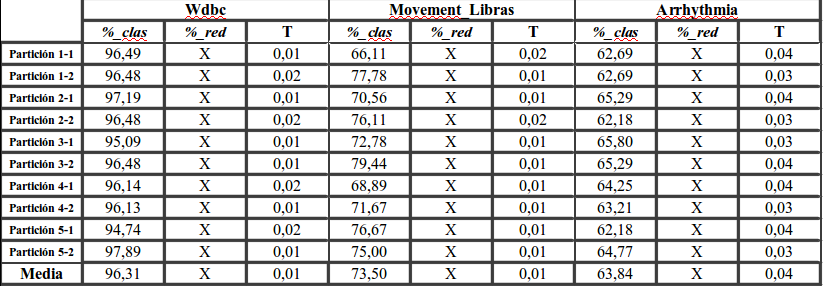
\includegraphics[width=1.0\linewidth]{3NN}
\caption{Experimentos para 3NN}
\label{fig:3NN}
\end{figure}

\begin{figure} [H]
	\centering
	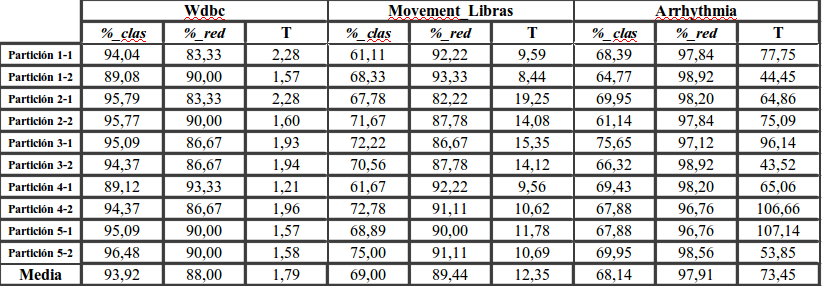
\includegraphics[width=1.0\linewidth]{SFS}
	\caption{Experimentos para SFS (algoritmo de comparación)}
	\label{fig:SFS}
\end{figure}

\begin{figure} [H]
\centering
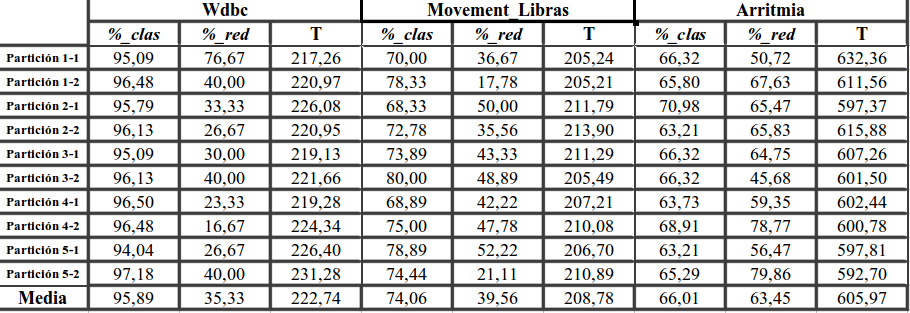
\includegraphics[width=1.0\linewidth]{AGG}
\caption{Experimentos para AGG}
\label{fig:AGG}
\end{figure}

\begin{figure} [H]
\centering
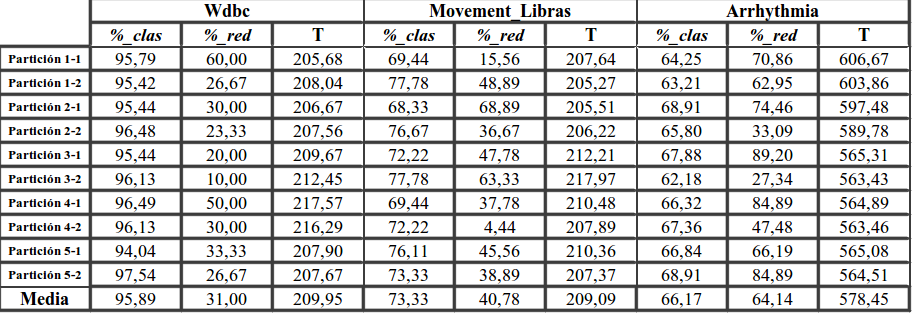
\includegraphics[width=1.0\linewidth]{AGE}
\caption{Experimentos para AGE}
\label{fig:AGE}
\end{figure}

\begin{figure} [H]
\centering
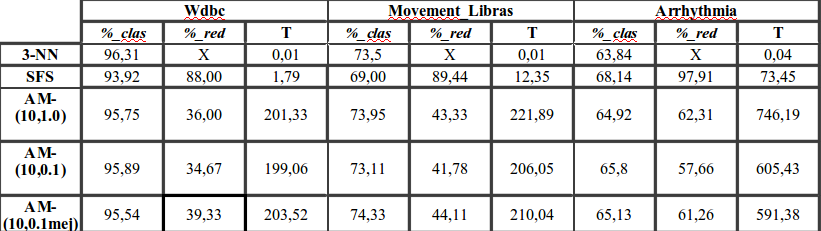
\includegraphics[width=1.0\linewidth]{todos}
\caption{Comparación de los algoritmos}
\label{fig:todos}
\end{figure}

Como vemos, los dos algoritmos genéticos mejoran a SFS en las dos primeras bases de datos. SFS no presenta apenas diversidad, por lo que probablemente caiga en un óptimo local pronto. Además, 3-NN nos muestra que para el vector de características completo, los resultados suelen ser mejores que con reducción sobre este, lo que podría significar que estas bases de datos tienen poco ruido en sus datos. Esto implica que una reducción más alta, como la que realiza SFS (pues la solución inicial que empieza a explotar es entera falsa), lleve hacia resultados peores que, en este caso, los algoritmos genéticos, que como vemos presentan menor tasa de reducción y mayor tasa de clase. Estos algoritmos, obviamente, presentan una mayor diversidad de exploración.
\\
\\
Lo mismo pasa para movement libras. Mientras SFS presenta una tasa de reducción del 89\%, AGG y AGE presentan una del 40\% aproximadamente ambas. Como podemos observar, estos dos algoritmos también nos da para esta base de datos un resultado de hasta un 5\% mejor que SFS (en tasa de clasificación).
\\
\\
Para Arrhythmia cambia bastante la cosa. 3NN obtiene un resultado del 63\% de tasa de clasificación, mientras que tras aplicar los algoritmos de búsqueda siempre solemos mejorar la tasa. Esto es un indicativo de que la base de datos contiene mucho ruido entre sus datos, por lo que la reducción de estos datos ruidosos mejora la tasa de clasificación. En este caso SFS sí se muestra mejor que AGG y AGE y también con una tasa de reducción mucho mejor (más de un 30\% superior), lo que nos puede llevar a la conclusión de que en este caso, empezar con una solución totalmente vacía nos llevará a soluciones mejores que comenzando con soluciones aleatorias (como hacemos en los algoritmos genéticos).
\\
\\
Como conclusión hay que decir que AGG y AGE probablemente obtendrían mejor resultado para Arrhythmia que SFS en el caso de que se empezara con una población algo más vacía, es decir, con vectores solución más vacíos, ya que como hemos visto en prácticas anteriores para Arrhythmia hay que reducir bastante el vector solución por ser tan ruidoso.
\\
\\
En cuanto a los tiempos, vemos como los algoritmos genéticos son mucho más lentos que SFS, algo normal cuando los genéticos van a realizar seguras 15000 evaluaciones de la función objetivo mientras que SFS probablemente acabe en un óptimo local mucho antes de llegar a ese número de evaluaciones. AGE es ligeramente más rápido que AGG y puede deberse a que en AGG se realizan más mutaciones y cruces y por esto esta diferencia temporal.
\\
\\
A continuación unos gráficos ilustrativos de la comparación de los algoritmos para cada base de datos.
\begin{figure} [H]
\centering
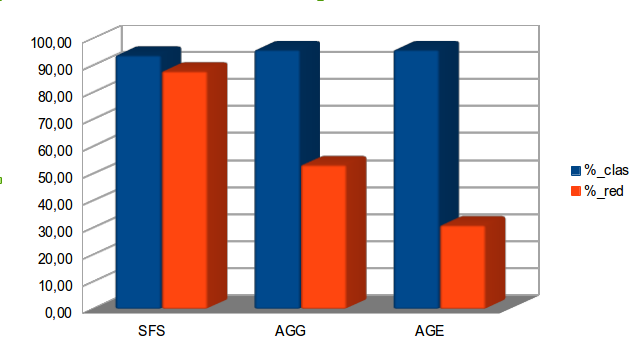
\includegraphics[width=1.0\linewidth]{graficaWDBC}
\caption{Gráfica comparativa para WDBC}
\label{fig:graficaWDBC}
\end{figure}

\begin{figure} [H]
\centering
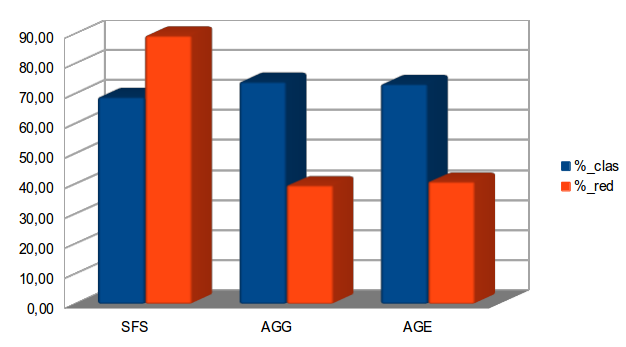
\includegraphics[width=1.0\linewidth]{graficaMovement}
\caption{Gráfica comparativa para movement libras}
\label{fig:graficaMovement}
\end{figure}

\begin{figure} [H]
\centering
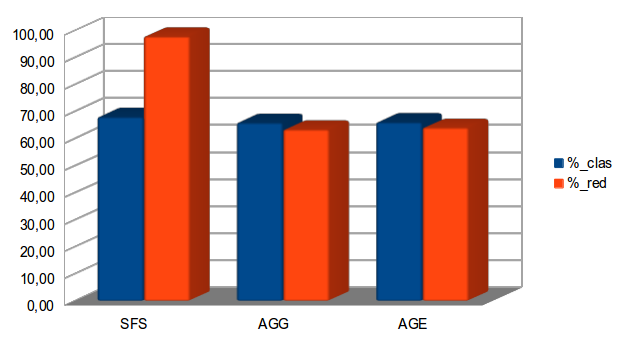
\includegraphics[width=1.0\linewidth]{graficaArrhythmia}
\caption{Gráfica comparativa para Arrhythmia}
\label{fig:graficaArrhythmia}
\end{figure}


\end{document}